\section{Results}
\par To validate the accuracy of MIDSX, validation simulations were performed and compared to reference data obtained by the American Association of Physicists in Medicine Task Group Report 195 (TG-195) \cite{sechopoulos_monte_2015}. The simulations performed from TG-195 were Case 1: "Half Value Layer," Case 2: "Radiography and Body Tomosynthesis," and Case 5: "CT with a Voxelized Solid." For Case 1, the primary air kerma was measured on a far away, circular ROI with a cone beam point source collimated such that all primary particles would be incident upon the ROI. The primary air kerma was measured with the domain filled only with air and then compared to the measured air kerma with an Al filter of thickness $t$ placed between the source and ROI. The ratios of the half value layer (HVL) and quarter value layer (QVL) primary air kerma to the primary background air kerma is represented by $R_1$ and $R_2$, respectively. By setting $t$ to correspond to the HVL and QVL for a particular spectrum, one can validate the material attenuation properties of an MC code system by comparing the simulated $R_1$ and $R_2$ to their theoretical values of 0.5 and 0.25, respectively. The simulation was performed for the monoenergetic energies of 30 keV and 100 keV, along with the polyenergetic spectrums of 30 kVp and 100 kVp, which were provided by TG-195. MIDSX's results for Case 1 agree to within 0.32\% of the mean results published by TG-195. The results of Case 1 are presented in Figure \ref{fig:HVLGraph}.
\par For Case 2, a full-field and pencil beam x-ray source were directed towards a cuboid tissue phantom at $0^\circ$ and $15^\circ$ with respect to the z-axis. Directly behind and inside the phantom, a grid of square ROIs and cube VOIs were placed, respectively. The simulation was performed for the TG-195 provided polyenergetic spectrum of 120 kVp and its mean energy of 56.4 keV. For the $0^\circ$, full-field ROI measurements not presented in this paper, a $<3$\% mean percent error (MPE) is seen for MIDSX's results to each ROI simulation. Furthermore, for the $0^\circ$ pencil-beam ROI measurements shown in Figure \ref{fig:ROIPGraph}, a $<2.1$\% MPE is observed for each ROI simulation except for the case of a single incoherent scatter. In this particular case, MIDSX's results for ROI 4 and 5 are significantly lower, with the MPE reaching 10\% for ROI 5. The full-field VOI energy deposition measurements depicted in Fig \ref{fig:BDGraph} show a minimal MPE of less than 0.1\% for the $0^\circ$ source. Conversely, for the MIDSX results at $15^\circ$, the MPE reaches an unexpectedly larger value of approximately 0.5\%.
\par For Case 5, a fan beam was collimated to the center of a voxelized human torso phantom provided by TG-195. To replicate a CT image, the simulation was repeated for several angles along a circle surrounding the phantom. The simulation was performed with Case 2's 120 kVp energy spectrum, and energy deposition was measured in the different materials/organs composing the phantom. Almost all of MIDSX's results for the $0^\circ$ source presented in Fig \ref{fig:CTGraph} are systematically lower than the mean of the reference code systems, with MPE's ranging from 1.1\% to 6.3\%. This pattern is disrupted by the thyroid, which is larger than the mean by 2.9\%. To quantify the cumulative error, the root mean square percent error (RMSPE) was calculated using each organ result, which resulted in the RMSPE for MIDSX being 5\%.   


\begin{figure}[htbp!]
    \centering
	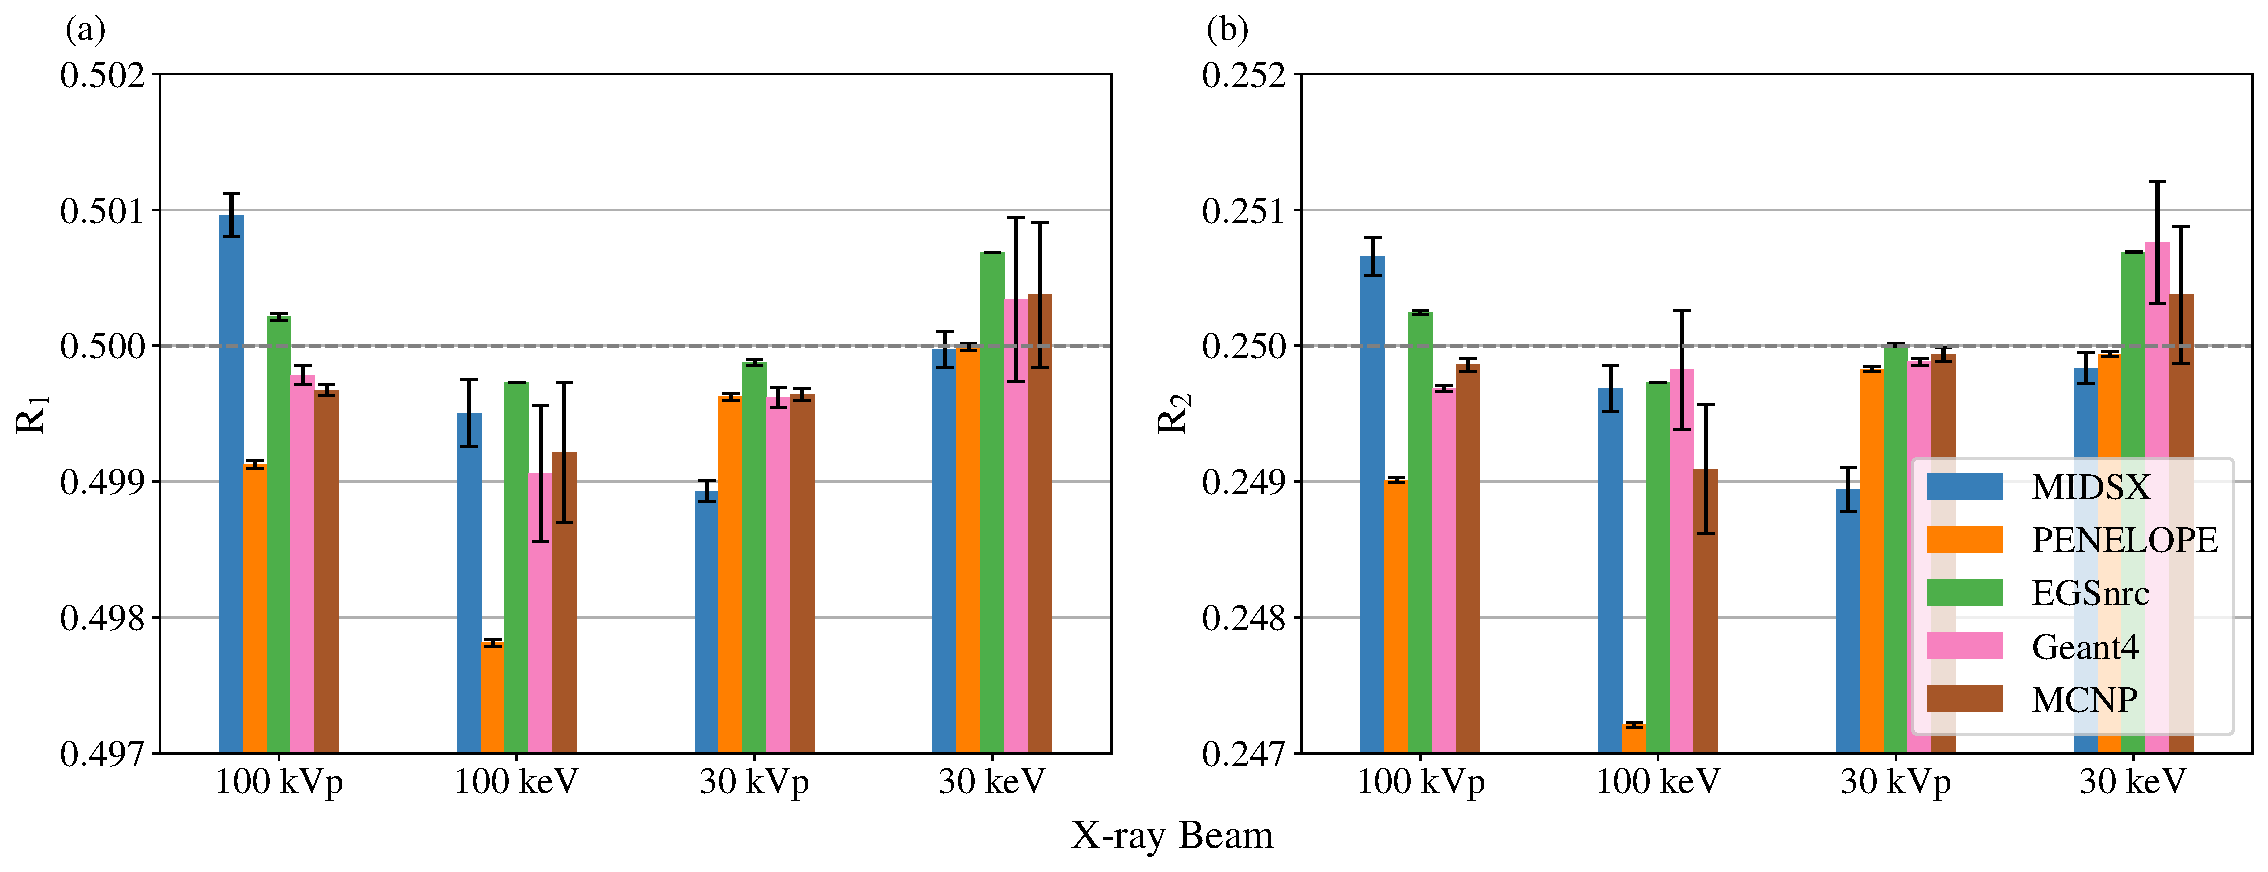
\includegraphics[width=1.0\textwidth]{../figures/HVL_and_QVL_paper_ready.pdf}
	\caption{Results for the (a) HVL and (b) QVL simulations as described by Case 1. The ratios of the primary HVL and QVL air kermas to the primary background air kermas is represented by $R_1$ and $R_2$, respectively. The simulation was performed for the monoenergetic energies 30 keV and 100 keV, along with the polyenergetic spectrums of 30 kVp and 100 kVp, which were provided by TG-195. A dashed-line is placed at $R_1 = 0.5$ and $R_2 = 0.25$ to aid the reader in comparing the simulated results to their theoretical counterpart.}
	\label{fig:HVLGraph}
\end{figure}

\begin{figure}[H]
    \centering
	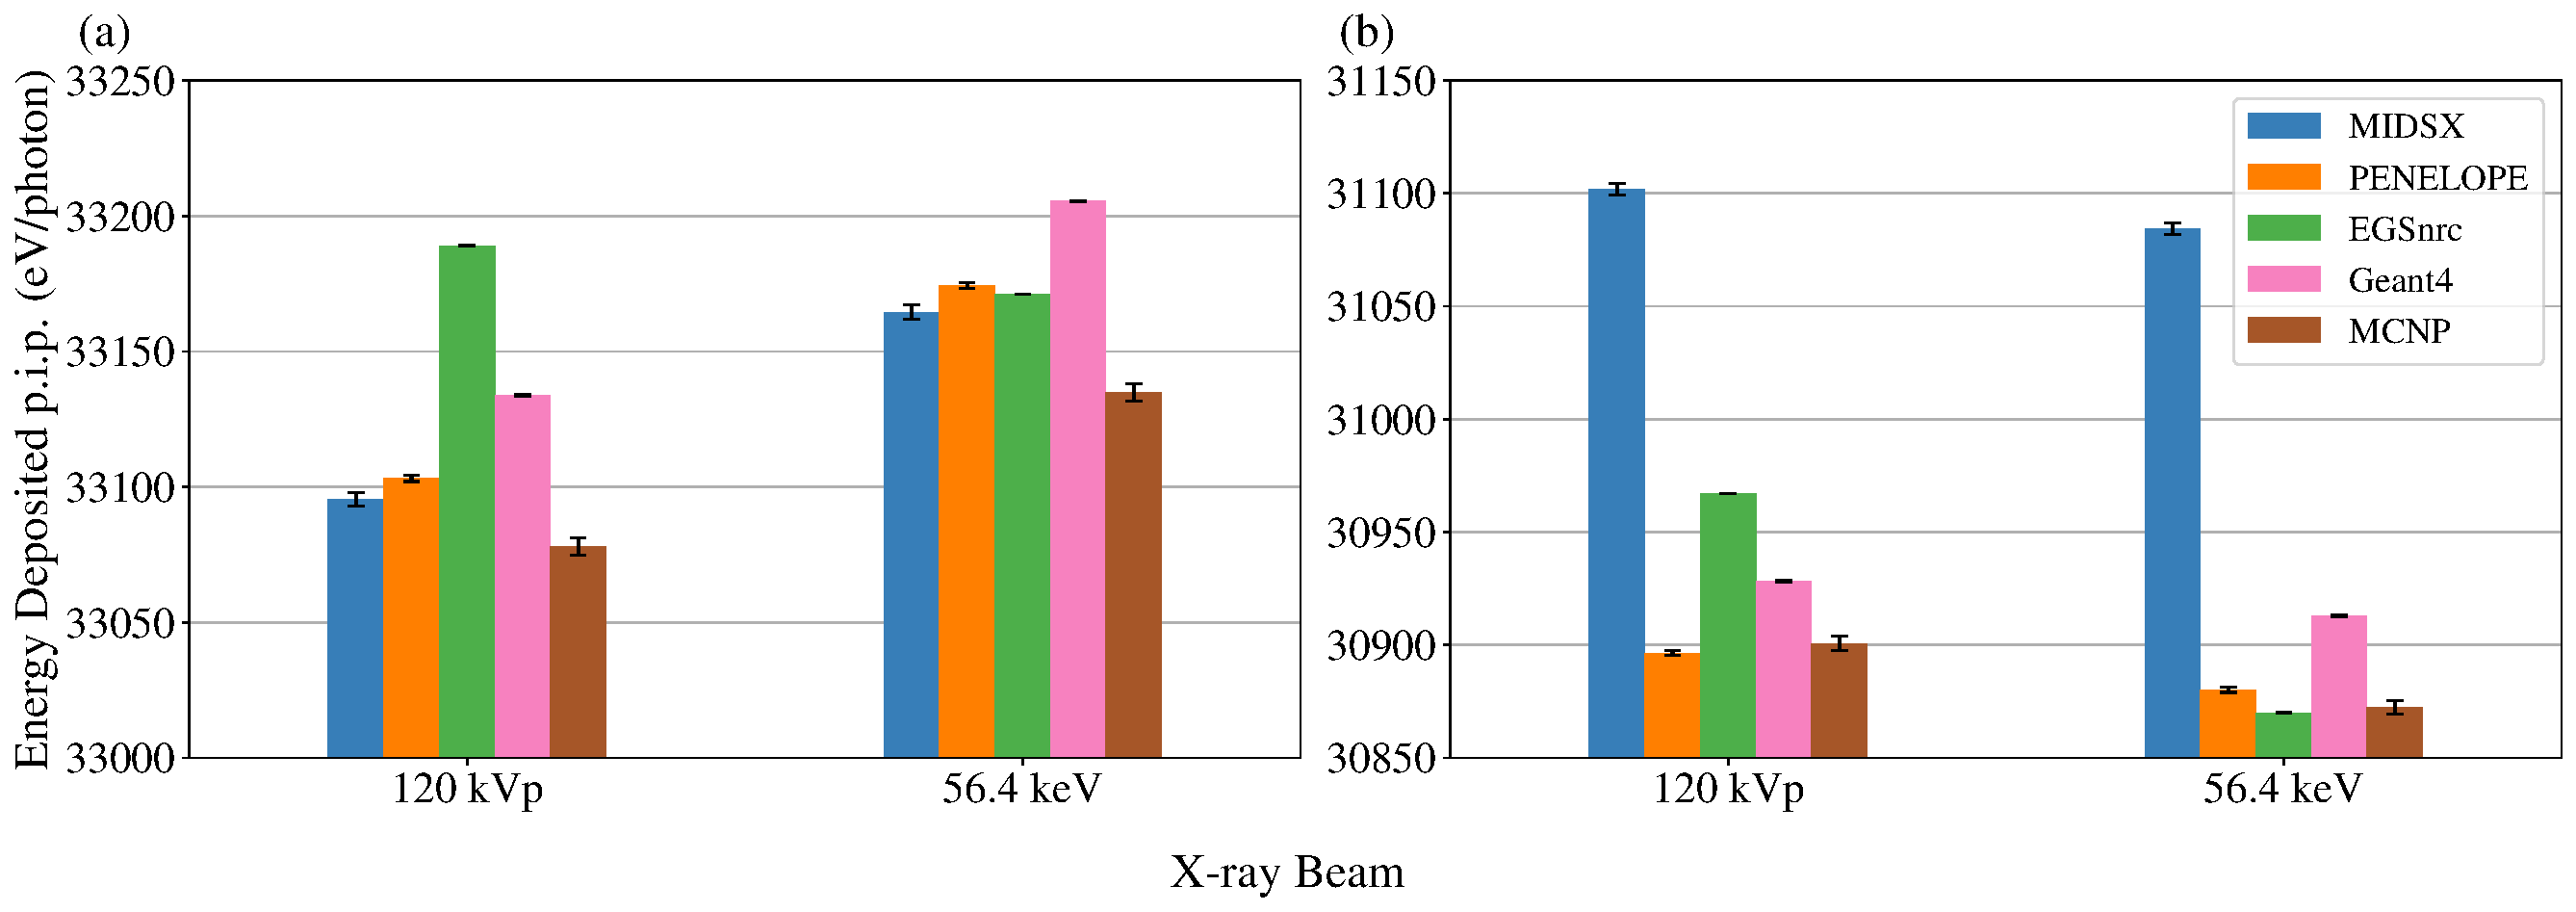
\includegraphics[width=1.0\textwidth]{../figures/radiography_body_dep_paper_ready.pdf}
	\caption{The energy deposited per initial photon (eV/photon) in the simulated tissue for the full-field simulation as described by Case 2. The simulation was performed at 56.4 keV and 120 kVp at both (a) $0^\circ$ and (b) $15^\circ$, with the 120 kVp spectrum provided by TG-195.}
 	\label{fig:BDGraph}
\end{figure}


\FloatBarrier


% \begin{figure}[htbp!]
%     \centering
% 	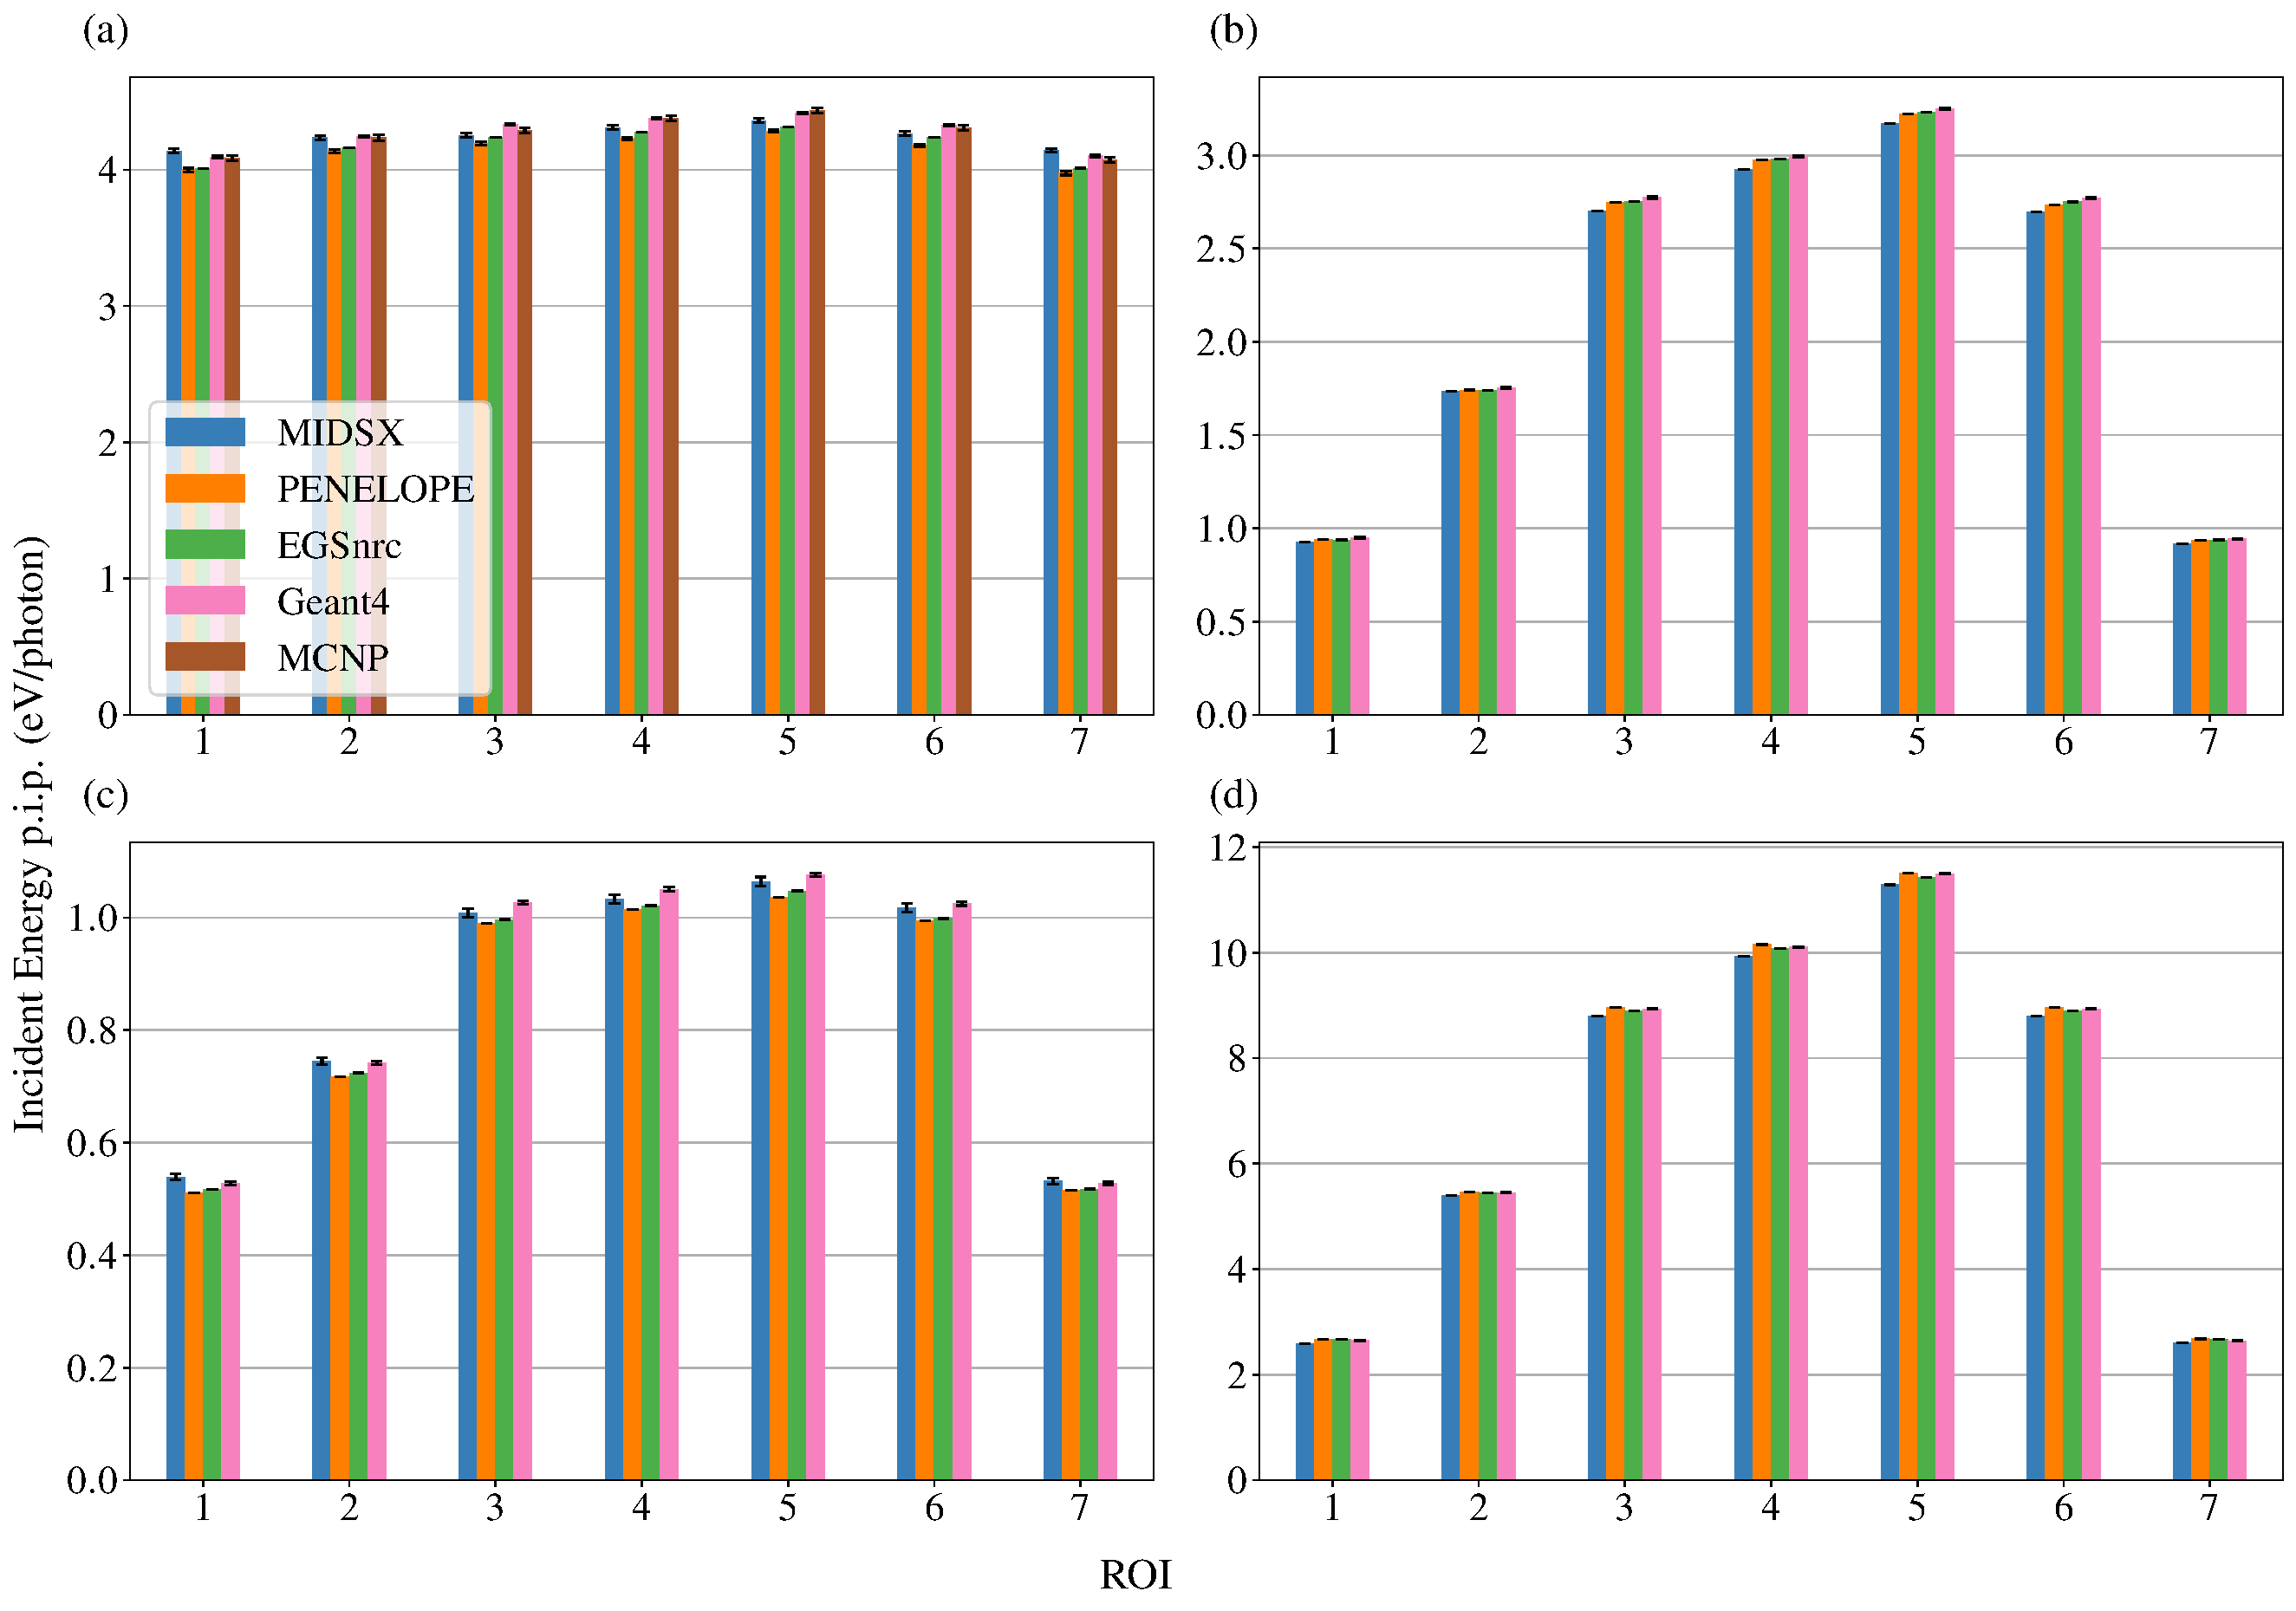
\includegraphics[width=1.0\textwidth]{../figures/ROI_0_deg_paper_ready.pdf}
% 	\caption{The energy per initial photon (eV/photon) of photons incident upon each region of interest (ROI) for the $0^\circ$, full-field, 56.4 keV simulation as described by Case 2. The incident energy was determined separately for photons that underwent (a) no real interactions, (b) a single incoherent scatter, (c) a single coherent scatter, (d) and multiple scatters.}
% 	\label{fig:ROIFFGraph}
% \end{figure}

\begin{figure}[htpb]
    \centering
	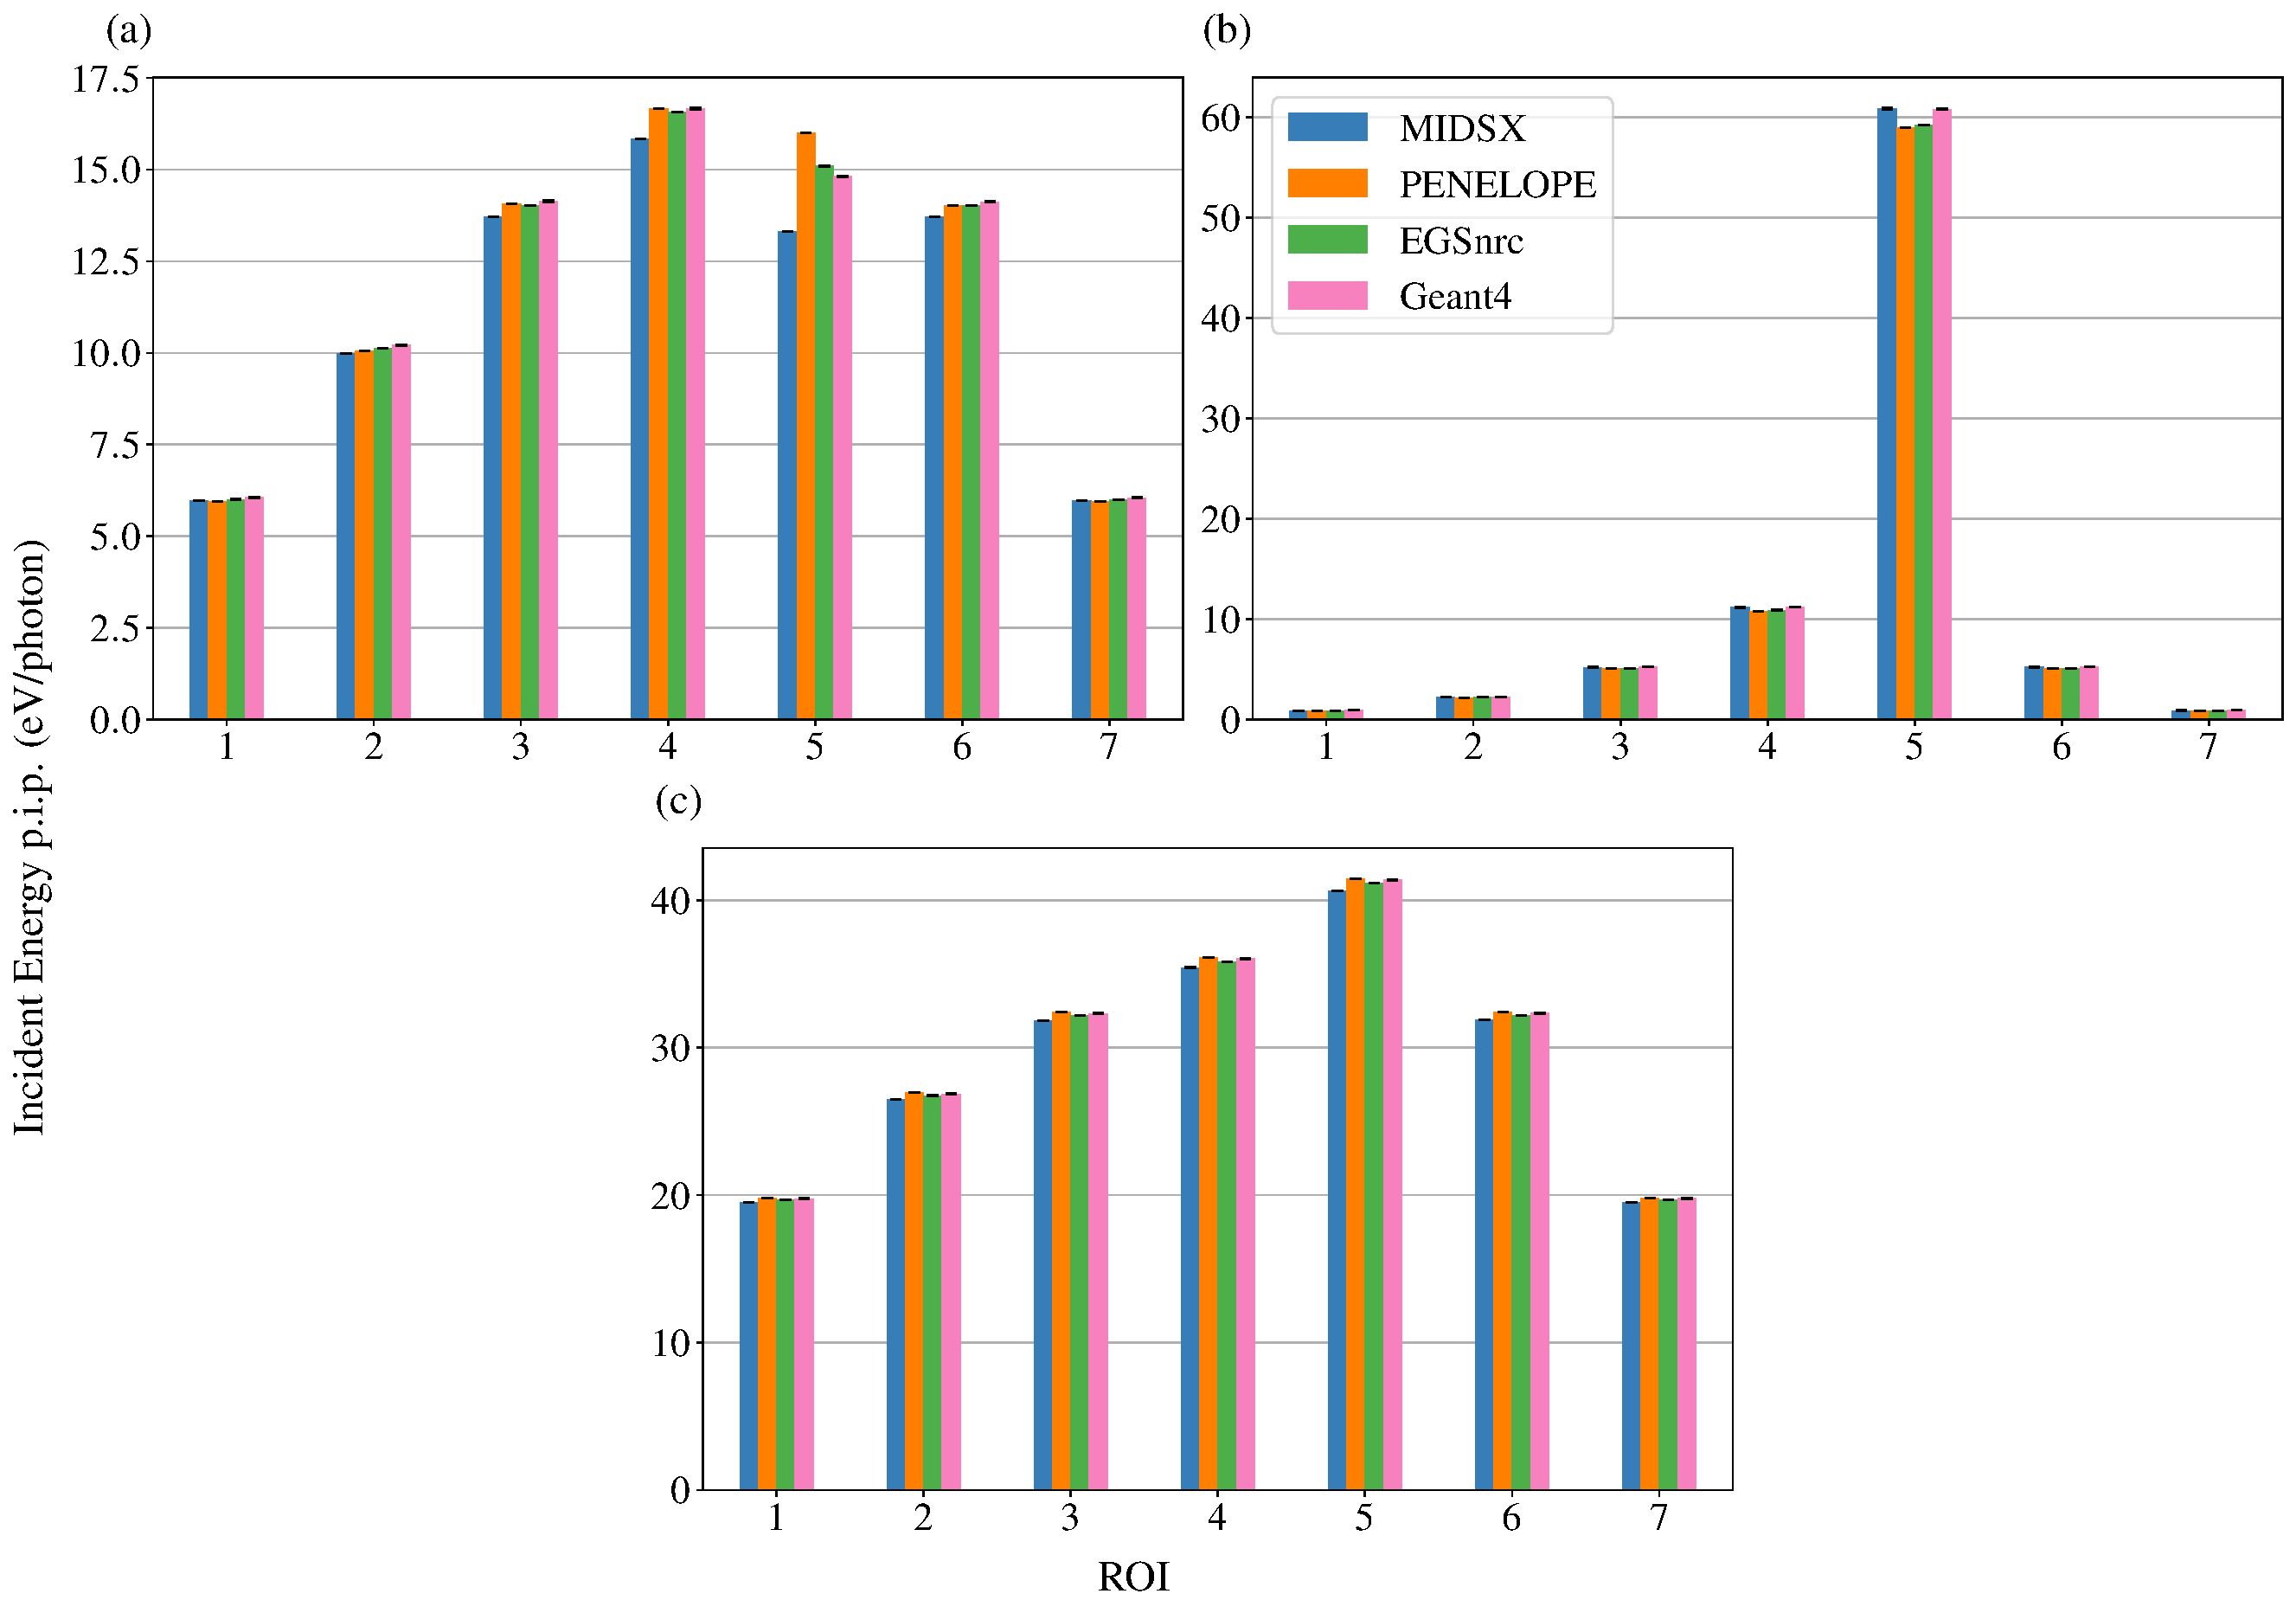
\includegraphics[width=0.98\textwidth]{../figures/ROI_0_deg_pencil_paper_ready.pdf}
	\caption{The energy per initial photon (eV/photon) of photons incident upon each region of interest (ROI) for the $0^\circ$, pencil beam, 56.4 keV simulation as described by Case 2. The incident energy was determined separately for photons that underwent (a) a single incoherent scatter, (b) a single coherent scatter, (c) and multiple scatters.}
	\label{fig:ROIPGraph}
\end{figure}

% \begin{figure}[H]
%     \centering
% 	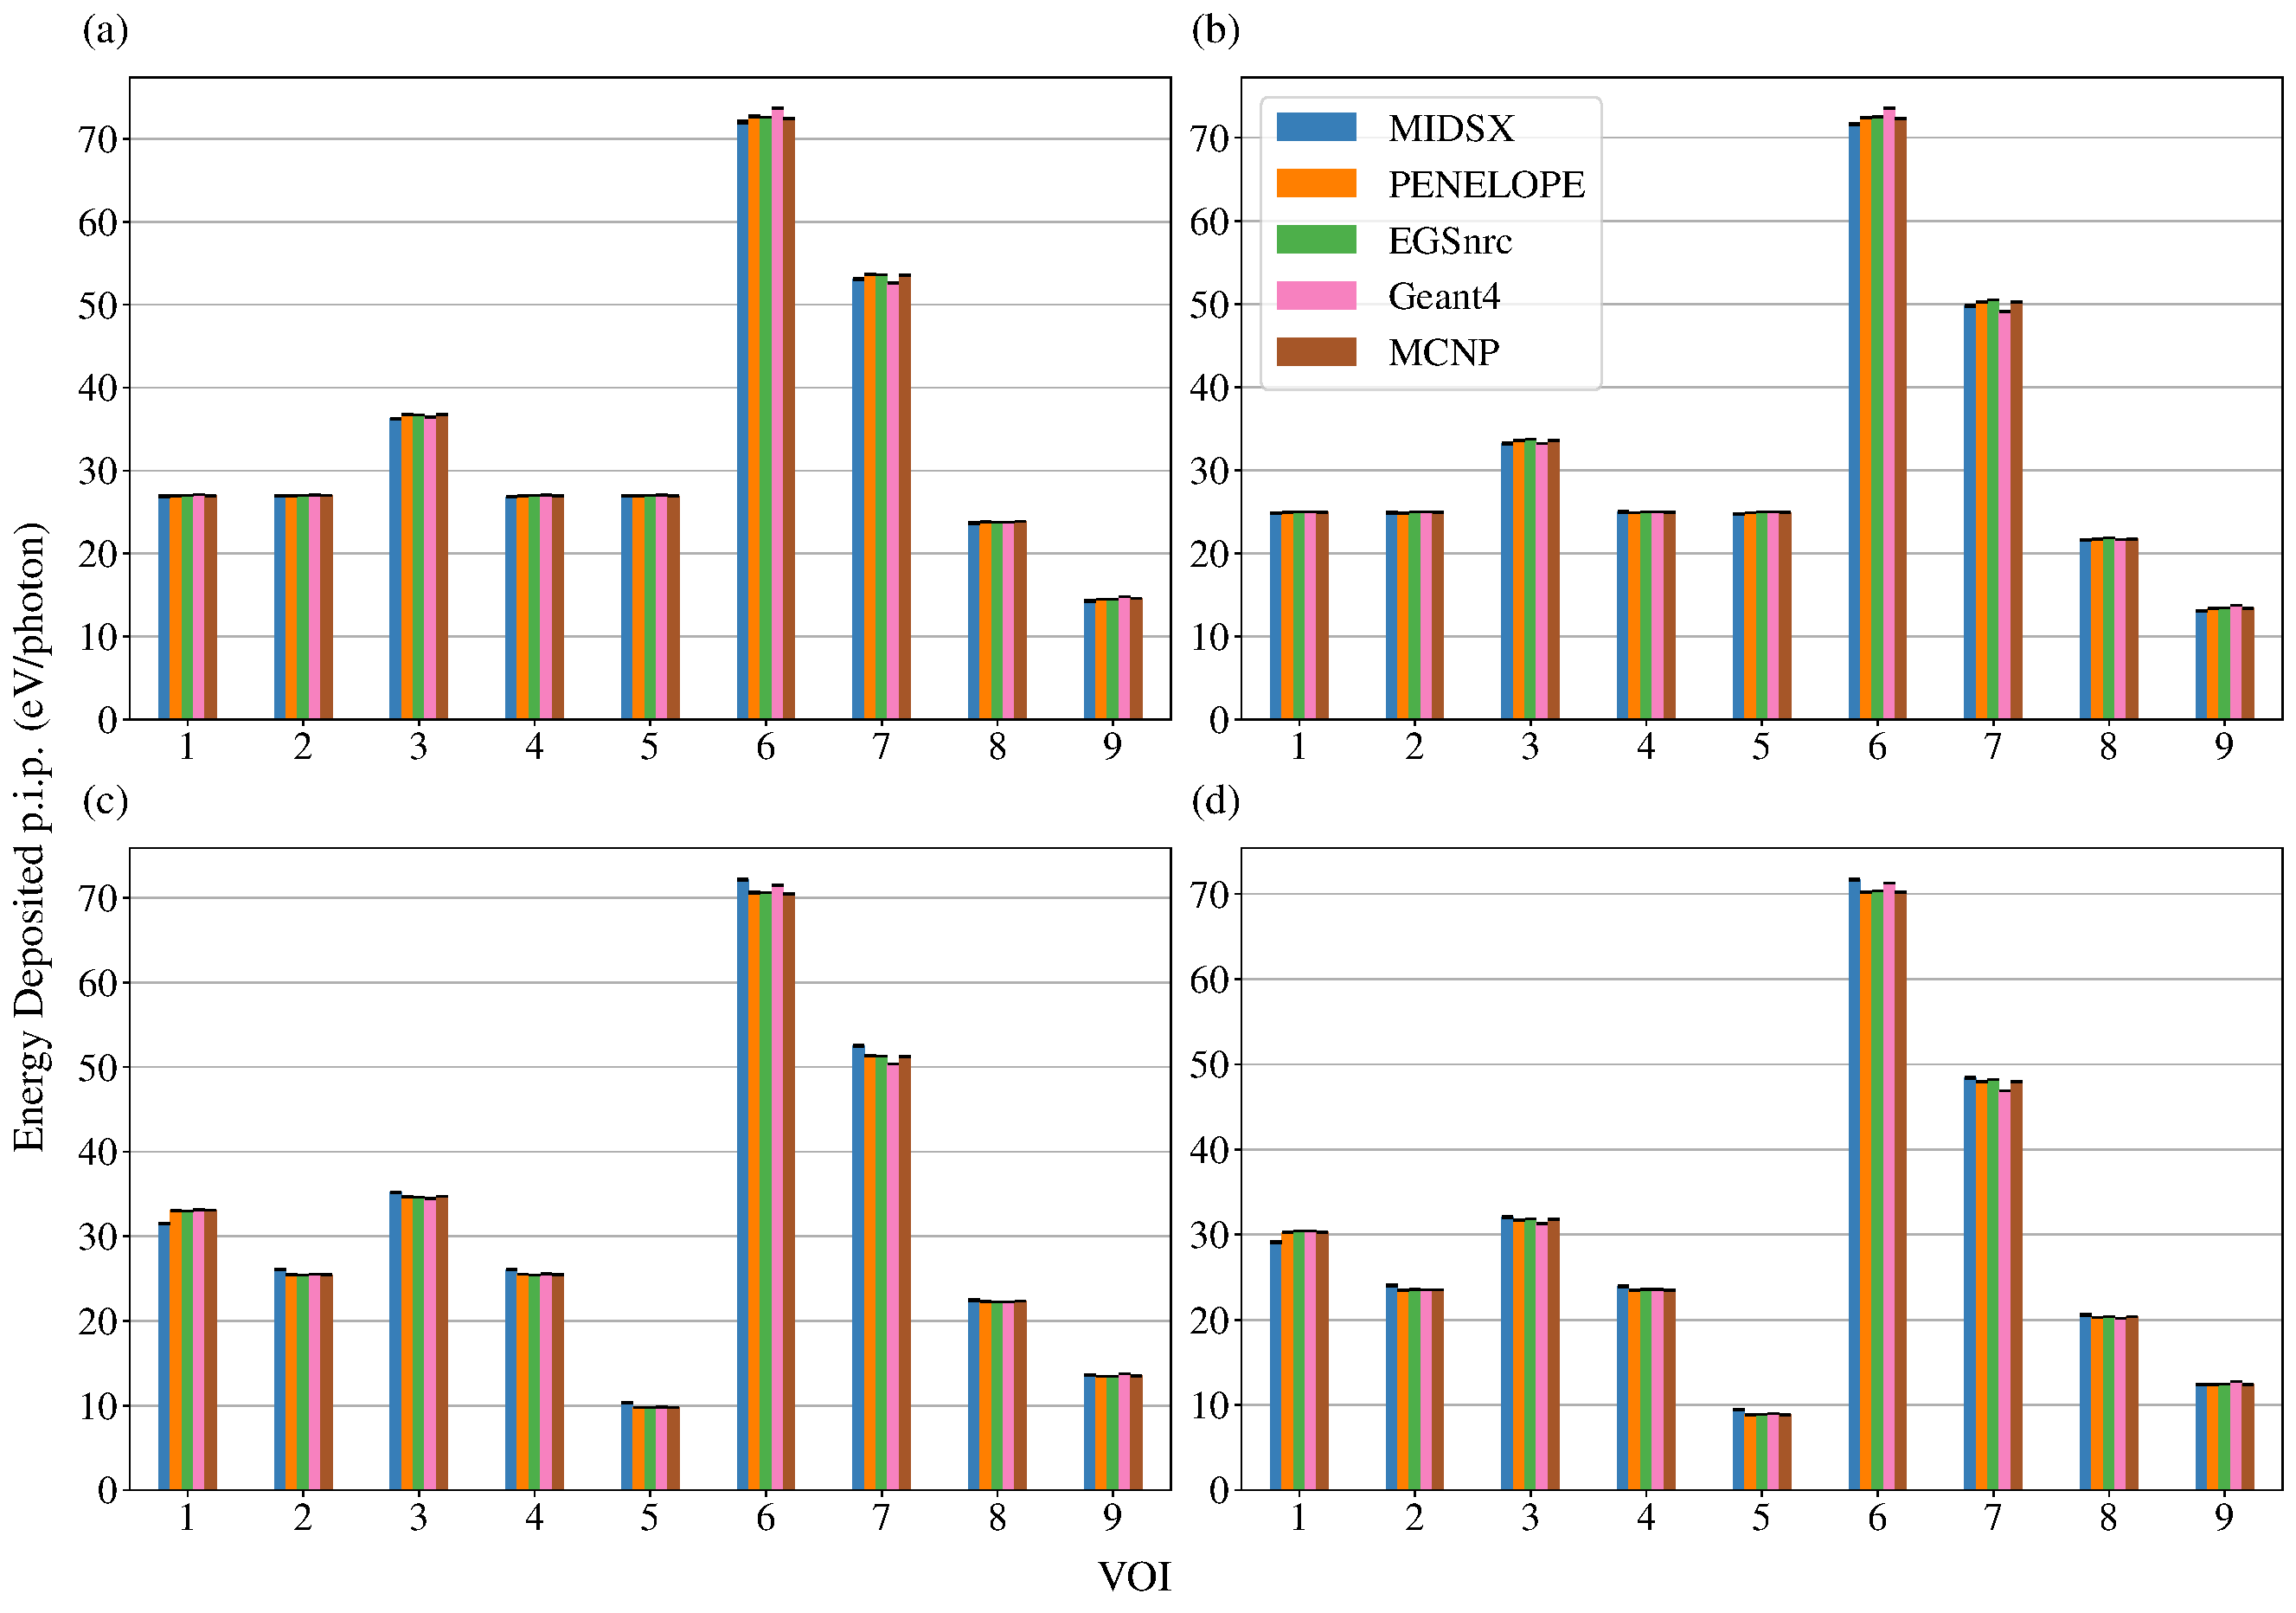
\includegraphics[width=1.0\textwidth]{../figures/VOI_paper_ready.pdf}
% 	\caption{The energy deposited per initial photon (eV/photon) in the volumes of interests (VOIs) for the full field simulation as described by Case 2. The simulation was performed at (a) $0^\circ$/56.4 keV, (b) $0^\circ$/120 kVp, (c) $15^\circ$/56.4 keV, and (d) $15^\circ$/120 kVp.}
% 	\label{fig:VOIFFGraph}
% \end{figure}

% \begin{figure}[H]
%     \centering
% 	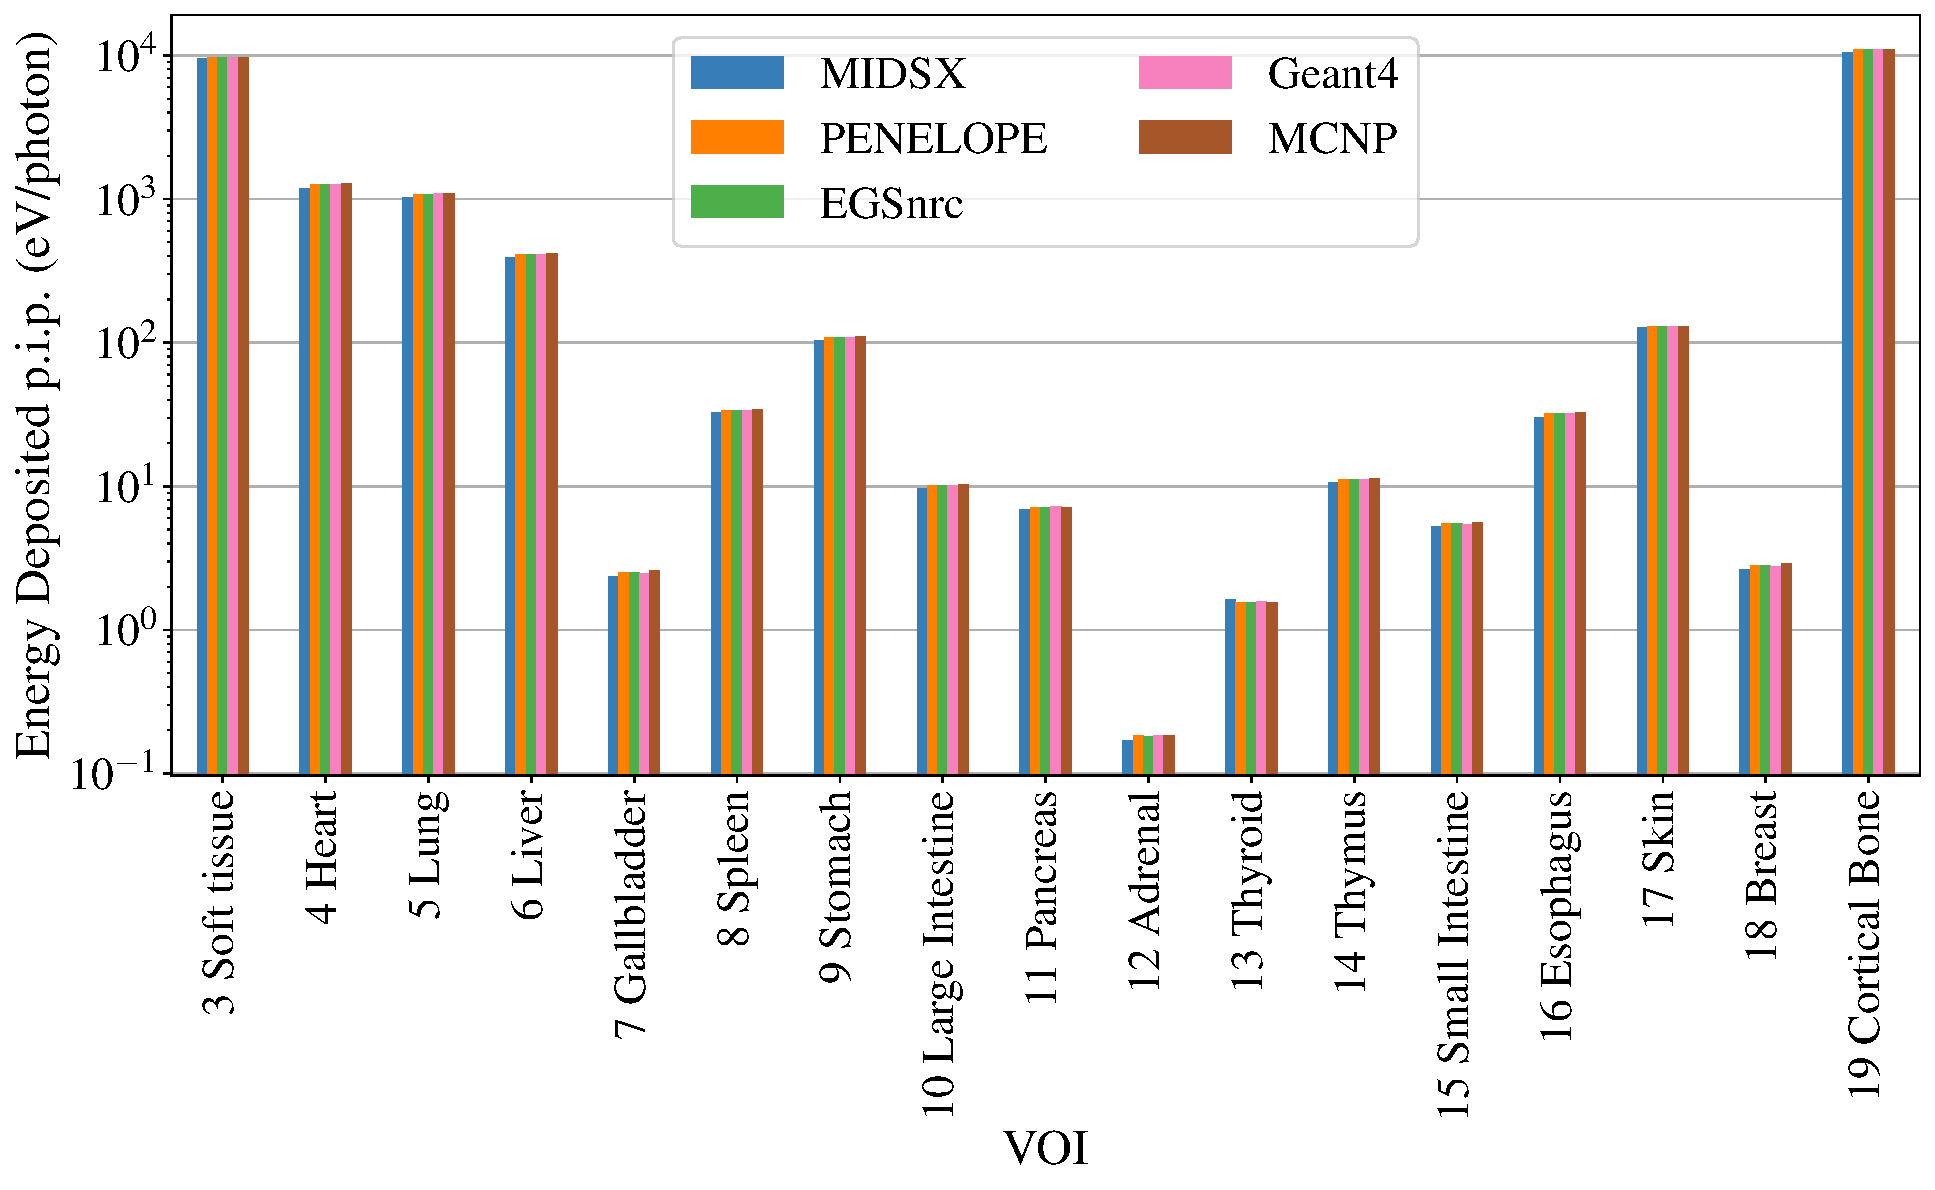
\includegraphics[width=1.0\textwidth]{../figures/CT_564_180.pdf}
% 	\caption{The energy deposited per initial photon (eV/photon) in the material IDs for the $180^\circ$, 56.4 keV simulation as described by Case 5.}
% 	\label{fig:CTGraph}
% \end{figure}

\begin{figure}[htbp]
    \centering
	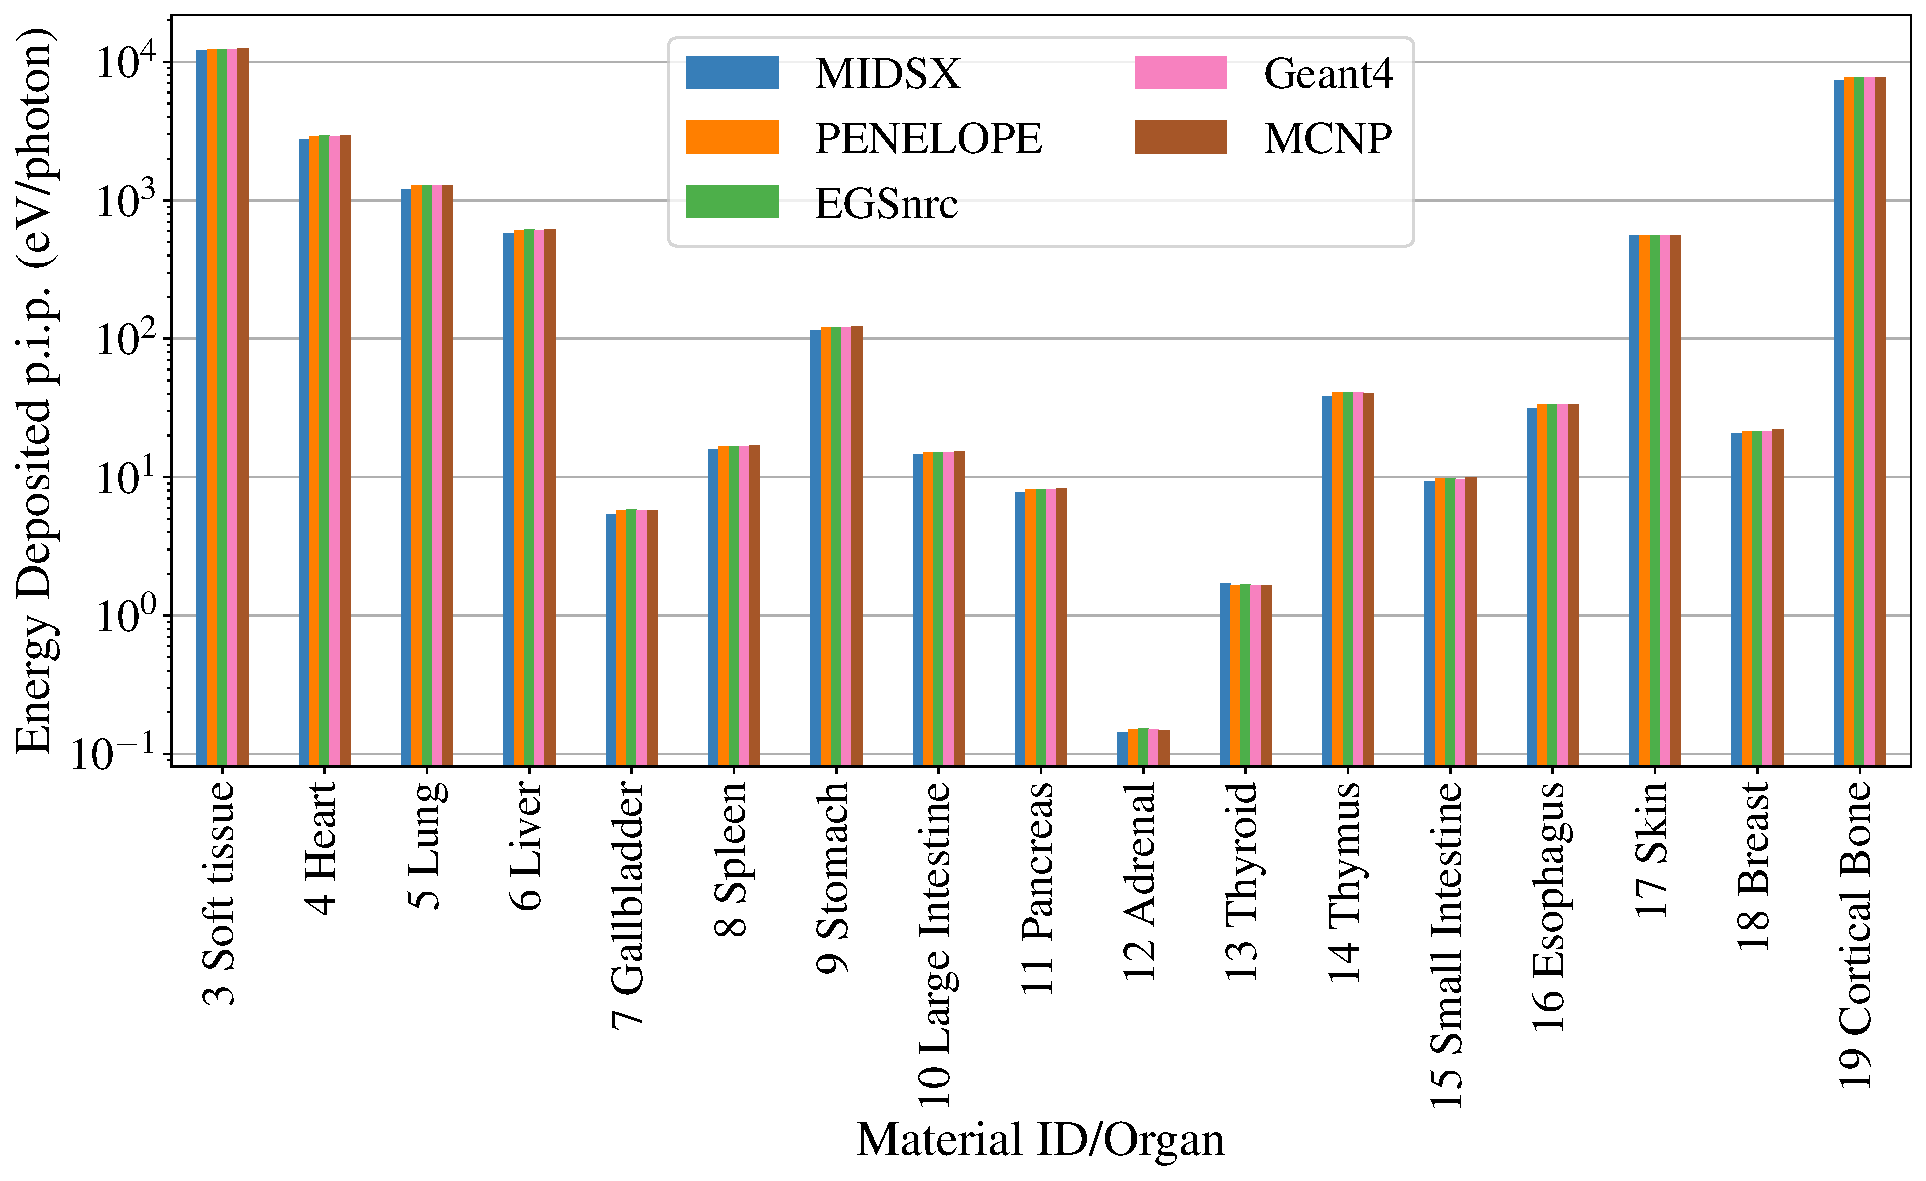
\includegraphics[width=0.8\textwidth]{../figures/CT_120_0.pdf}
	\caption{The energy deposited per initial photon (eV/photon) in the material IDs/organs composing a voxelized human phantom for the $0^\circ$, 120 kVp simulation as described by Case 5.}
	\label{fig:CTGraph}
\end{figure}

\FloatBarrier
